\documentclass[11pt]{beamer}
\usepackage{amsmath,amssymb}
\usepackage{graphicx}
\usepackage{url}
\usepackage{textcomp}

\usetheme{iqss}


\title[Beamer Demo]{Beamer Class Demonstration\thanks{Thanks to all the Beamer people!}}

\author{Me Myself}
\date{\today}
\institute{IQSS}
\titlegraphic{
\includegraphics[width=4cm]{iqlogo.png}}

\begin{document}

\begin{frame}
  \maketitle
\end{frame}

\begin{frame}
  \frametitle{Overview}
  \tableofcontents
\end{frame}

\section{Beamer Features}

\subsection{Some of Gary's Examples}

\begin{frame}\frametitle{What's this course about?}
  \begin{itemize}
  \item \alert{Specific statistical methods for many research problems}
    \begin{itemize}
    \item How to learn (or create) new methods
    \item Inference: \underline{Using facts you know to learn about
        facts you don't know}
    \end{itemize}
  \item \alert{How to write a publishable scholarly paper}
  \item \alert{All the practical tools of research} --- theory,
    applications, simulation, programming, word processing, plumbing,
    whatever is useful
  \item $\leadsto$ \alert{Outline and class materials:}
    \begin{itemize}
    \item[]    \begin{center}
      \mbox{{\huge\parbox[b][.5in][t]{1in}{\alert{j.mp/G2001}}}
        $\qquad\qquad$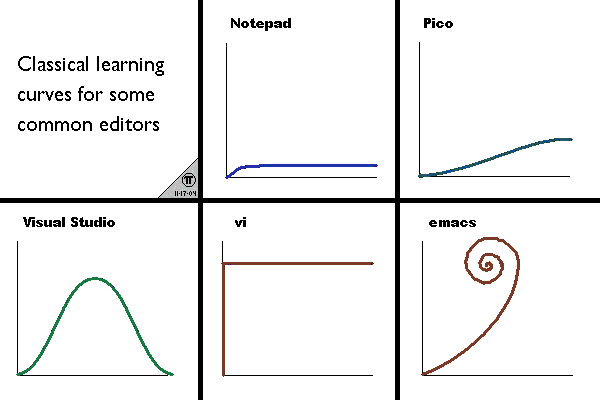
\includegraphics[width=.95in]{figs/phbAr.png}}
    \end{center}
  \item The syllabus gives topics, not a weekly plan.
  \item We will go as fast as possible subject to everyone following
    along
  \item We cover different amounts of material each week
  \end{itemize}
  \end{itemize}
\end{frame}


\begin{frame}\frametitle{How much math will you scare us with?}
  \begin{itemize}
  \item All math requires two parts: \alertb{proof} and
    \alertb{concepts \& intuition}
  \item Different classes emphasize:
    \begin{itemize}
    \item \alert{Baby Stats}: dumbed down proofs, vague intuition
    \item \alert{Math Stats}: rigorous mathematical proofs
    \item \alert{\underline{Practical Stats}}: deep concepts and
      intuition, proofs when needed
      \begin{itemize}
      \item Goal: how to do empirical research, in depth
      \item Use rigorous statistical theory --- when needed
      \item Insure we understand the intuition --- always
      \item Always traverse from theoretical foundations to practical
        applications
      \item Includes ``how to'' computation
      \item $\leadsto$ Fewer proofs, more concepts, better practical
        knowledge
      \end{itemize}
    \end{itemize}
  \item Do you have the background for this class? \uncover<+->{\alert{A
      Test: What's this?
    \begin{align*}
      b=(X'X)^{-1}X'y
    \end{align*} }}
  \end{itemize}
\end{frame}

\begin{frame}\frametitle{Systematic Components: Examples}
  \begin{center}
    \includegraphics<+->[width=8cm]{figs/functionalForms}
  \end{center}
  \begin{itemize}
  \item \alertb{$E(Y_i) \equiv \mu_i = X_i\beta = \beta_0 +
      \beta_1X_{1i} +\dots+\beta_kX_{ki}$}
  \item \alertc{$\Pr(Y_i=1) \equiv \pi_i =
      \frac{1}{1+e^{-x_i\beta}}$}
  \item \alertd{$V(Y_i)\equiv \sigma_i^2 = e^{x_i\beta}$}
  \item Interpretation:
    \begin{itemize}
    \item Each is a \alert{class of functional forms}
    \item Set $\beta$ and it picks out one \alert{member of the class}
    \item \alert{$\beta$} in each is an ``effect parameter'' vector,
      with different meaning
    \end{itemize}    
  \end{itemize}
\end{frame}


\begin{frame}\frametitle{Negative Binomial Derivation} \uncover<+->{Recall:}
  \begin{equation*}
    \uncover<+->{\Pr(A|B)=\frac{\Pr(AB)}{\Pr(B)} \implies \alertb{\Pr(AB)}=\alerte{\Pr(A|B)}\alertd{\Pr(B)}}
  \end{equation*}
  \begin{align*}
    \uncover<+->{\text{NegBin}(y|\phi,\sigma^2) &= \int_0^\infty
      \alerte{\text{Poisson}(y|\lambda)}
      \times\alertd{\text{gamma}(\lambda|\phi,\sigma^2)}d\lambda\\}
    \uncover<+->{&= \int_0^\infty
      \alertb{\P(y,\lambda|\phi,\sigma^2) }d\lambda\\}
    \uncover<+->{&=
      \frac{\Gamma\left(\frac{\phi}{\sigma^2-1}+y_i\right)}
      {y_i!\Gamma\left(\frac{\phi}{\sigma^2-1}\right)}
      \left(\frac{\sigma^2-1}{\sigma^2}\right)^{y_i}
      \left(\sigma^2\right)^{\frac{-\phi}{\sigma^2-1}}}
  \end{align*}
\end{frame}


\subsection{Structural Features}

\begin{frame}
  \frametitle{Structural Features}
  \begin{block}{Levels of Structure}
    \begin{itemize}
      \item usual \LaTeX\ \textbackslash{}section, \textbackslash{}subsection 
      commands
      
      \item `frame' environments provide slides
      
      \item `block' environments divide slides into logical sections
      
      \item `columns' environments divide slides vertically (example later)
      
      \item overlays (\`a la prosper) change content of slides dynamically
    \end{itemize}
  \end{block}
  
  \begin{example}[Overlay Alerts]
    On the first overlay, \alert<1>{this text} is highlighted (or \emph{alerted}).\\ On the second, \alert<2>{this text} is.
  \end{example}
\end{frame}

\begin{frame}
  \frametitle{Alerts}
  \begin{itemize}
     \item First level \alert{alert}
     \item Second level \alertb{alert}
     \item Third level \alertc{alert}
     \item Fourth level \alertd{alert}
     \item Fifth level \alerte{alert}
  \end{itemize}

\end{frame}
  

\subsection{Other Features}

\begin{frame}
  \frametitle{Other Features}

  \begin{block}{Levels of Structure}
    \begin{itemize}
      \item Clean, extensively customizable visual style
      
      \item No weird scaling like prosper
      \begin{itemize}
        \item slides are 96~mm~$\times$~128~mm
        
        \item text is 10-12pt on slide
        
        \item slide itself magnified with Adobe Reader/xpdf/gv to fill screen
      \end{itemize}
      
      \item pgf graphics framework easy to use
      
      \item include external JPEG/PNG/PDF figures
      
      \item output directly to pdf: no PostScript hurdles
      
      \item detailed User's Manual (with good presentation advice, too)
    \end{itemize}
  \end{block}
\end{frame}

\subsection{Blocks}

\begin{frame}
\frametitle{Theorems and Proofs}
\framesubtitle{The proof uses \textit{reductio ad absurdum}.}
\begin{theorem}
There is no largest prime number.
\end{theorem}
\begin{proof}
\begin{enumerate}
\item<1-| alert@1> Suppose $p$ were the largest prime number.
\item<2-> Let $q$ be the product of the first $p$ numbers.
\item<3-> Then $q+1$ is not divisible by any of them.
\item<1-> But $q + 1$ is greater than $1$, thus divisible by some prime
number not in the first $p$ numbers.\qedhere
\end{enumerate}
\end{proof}
\end{frame}


\begin{frame}
  \frametitle{Blocks}

  \begin{block}{Normal block}
A \alert{set} consists of elements.
\end{block}

\begin{alertblock}{Alert block}
$2=2$.
\end{alertblock}

\begin{exampleblock}{Example block}
The set $\{1,2,3,5\}$ has four elements.
\end{exampleblock}

\end{frame}

\end{document}

%%% Local Variables:
%%% mode: latex
%%% TeX-master: t
%%% End:
